\documentclass[12pt]{article}
\usepackage[spanish]{babel}
\usepackage[utf8]{inputenc}
\usepackage{graphicx}
\usepackage{hyperref}
\usepackage{booktabs}
\usepackage{multirow}
\usepackage{amsmath}
\usepackage{float}
\usepackage[document]{ragged2e}
\usepackage{microtype}
\addto\captionsspanish{%
  \renewcommand{\tablename}{Tabla}%
}



\usepackage[a4paper, margin=2.5cm]{geometry}

% Configuración de encabezado
\usepackage{fancyhdr}
\pagestyle{fancy}
\fancyhf{}
\lhead{Análisis predictivo del precio de Bitcoin usando modelos de Deep Learning}
\rfoot{Página \thepage}

\title{
    \vspace{-2cm}
    \normalsize \textbf{Universidad de Buenos Aires} \\
    \textbf{Laboratorio de Sistemas Embebidos} \\
    \textbf{Especialización en Inteligencia Artificial} \\
    \vspace{0.5cm}
    {Trabajo Práctico Final} \\
    \vspace{1cm}
    \Large \textbf{Análisis predictivo del precio de Bitcoin usando modelos de Deep Learning} \\
    \vspace{1cm}
    \large Docente: Dr. Camilo Argoty
    \vspace{1cm}
}
\author{
    Noelia Melina Qualindi \\
    Jorge Valdez \\
    Fabián Sarmiento \\
    Matías Marando
    \vspace{1cm}
}
\date{\today}

\begin{document}
\justifying  % Apply to whole document from this point
\maketitle

%%%%%%%%%%%%%%%%%%%%%%%%%%%%%%%%%%%%%%%%%%%%%%%%%%%%%%%%%%%%%%%%%%%%%%%%

\begin{abstract}
Este trabajo presenta un análisis comparativo de modelos avanzados de deep learning para la predicción del precio de Bitcoin (BTC-USD). Se implementaron y evaluaron cuatro arquitecturas:  Transformer Vanilla para series temporales, TFT (\textit{Temporal Fusion Transformer}), Informer y  NHiTS (\textit{Neural Hierarchical Interpolation for Time Series}), utilizando datos históricos desde 2012 hasta la fecha.
Los resultados demuestran que los modelos pueden capturar patrones complejos en los datos. % TODO con el <mejor modelo> alcanzando un MAE de <??> en el conjunto de prueba.
El estudio incluye un análisis exhaustivo de preprocesamiento, diseño de modelos y validación de resultados, concluyendo con recomendaciones para futuras mejoras.
\end{abstract}

%%%%%%%%%%%%%%%%%%%%%%%%%%%%%%%%%%%%%%%%%%%%%%%%%%%%%%%%%%%%%%%%%%%%%%%%

\newpage
\section{Introducción}
\label{sec:intro}

%Las criptomonedas, particularmente Bitcoin, presentan desafíos únicos para el análisis predictivo debido a su alta volatilidad y sensibilidad a factores externos. Este trabajo busca responder:


Las criptomonedas han emergido como una clase de activos revolucionaria que ha transformado el panorama financiero global desde la introducción de Bitcoin en 2009. Particularmente Bitcoin, como la primera y más establecida criptomoneda, presenta desafíos únicos y complejos para el análisis predictivo que la distinguen significativamente de los activos financieros tradicionales.

La naturaleza descentralizada de Bitcoin, combinada con su extrema volatilidad de precios, crea un entorno de trading caracterizado por fluctuaciones dramáticas que pueden superar el 10-20\% en períodos de 24 horas. Esta volatilidad intrínseca se ve amplificada por múltiples factores: la alta sensibilidad a noticias regulatorias, eventos geopolíticos, decisiones de grandes instituciones, movimientos de "ballenas" (grandes tenedores), cambios en la percepción pública, y la influencia de redes sociales y figuras públicas influyentes.
%Desafíos para el modelado predictivo:
A diferencia de los mercados financieros tradicionales, Bitcoin opera en un mercado global 24/7 sin interrupciones, lo que genera patrones temporales únicos y ausencia de los típicos efectos de cierre de mercado. Además, la relativa juventud del mercado cripto significa que los modelos deben adaptarse a un ecosistema en constante evolución con datos históricos limitados comparados con mercados centenarios.
%Motivación y objetivos del estudio:
Dada la creciente adopción institucional de Bitcoin y su integración en portafolios de inversión \textit{mainstream}, existe una necesidad crítica de desarrollar modelos predictivos robustos que puedan manejar estas características únicas. Este trabajo busca responder el siguiente planteamiento:


\begin{center}
\fbox{
\begin{minipage}{0.9\textwidth}
¿Pueden los modelos modernos de deep learning predecir efectivamente el precio de Bitcoin a corto plazo, y cómo se comparan diferentes arquitecturas en este contexto?
\end{minipage}
}
\end{center}

%%%%%%%%%%%%%%%%%%%%%%%%%%%%%%%%%%%%%%%%%%%%%%%%%%%%%%%%%%%%%%%%%%%%%%%%

\newpage
\section{Metodología}
\label{sec:metodologia}

\subsection{Datos Utilizados}
%El dataset contiene:
El dataset empleado presenta las siguientes característcias:

\begin{itemize}
\item \textbf{Fuente}: Kaggle (Bitcoin Historical Data)
\item \textbf{Período}: 2020-01-01 a 2023-12-31 
\item \textbf{Variables utilizadas}:
\begin{table}[H]
\centering
\begin{tabular}{ll}
\toprule
\textbf{Variable} & \textbf{Descripción} \\
\midrule
Timestamp & Fecha en formato UNIX \\
Close & Precio de cierre (USD) \\
\bottomrule
\end{tabular}
\end{table}
\end{itemize}

%%%%%%%%%%%%%%%%%%%%%%%%%%%%%%%%%%%%%%%%%%%%%%%%%%%%%%%%%%%%%%%%%%%%%%%%

\bigskip
\subsection{Preprocesamiento}

El preprocesamiento de los datos se realizó en varias etapas clave:

\begin{enumerate}
\item \textbf{Limpieza de datos}: Se comenzó renombrando las columnas relevantes para facilitar su uso posterior,
en particular la marca temporal y el precio de cierre. Luego, se eliminaron todas las filas que contenían valores nulos en la columna del precio, asegurando que todos los datos utilizados para el análisis fuesen válidos.

\item \textbf{Conversión de tiempo}: La columna de tiempo original, que venía en formato UNIX (segundos desde 1970), fue convertida a un formato de fecha estándar para su correcta interpretación y manipulación.

\item \textbf{Ordenamiento temporal}: Se ordenaron los datos cronológicamente según la fecha, para asegurar la coherencia temporal en los análisis y predicciones.

\item \textbf{Resampleo diario}: Dado que los datos originales tenían una granularidad de un minuto,
se procedió a realizar un promedio diario del precio, lo cual reduce la variabilidad y permite un análisis más robusto en horizontes temporales más amplios.

\item \textbf{Normalización}: Se aplicó una normalización de tipo Min-Max al precio diario, escalando los valores al rango [0, 1].
Esto facilitó el entrenamiento de los modelos de \textit{deep learning}, ya que evita problemas numéricos asociados a diferentes escalas.

\item \textbf{Creación de secuencias}: Para poder alimentar los modelos, los datos fueron transformados en ventanas deslizantes.
Se definieron tres longitudes de entrada de: 90, 180 y 365 días y un horizonte de predicción de 10 días.
Cada muestra consiste en una secuencia de precios normalizados para entrenar el modelo a predecir el comportamiento futuro.
\end{enumerate}

%%%%%%%%%%%%%%%%%%%%%%%%%%%%%%%%%%%%%%%%%%%%%%%%%%%%%%%%%%%%%%%%%%%%%%%%

\newpage
\subsection{Modelos Implementados}


%Se implementaron tres modelos de predicción de series temporales utilizando distintas arquitecturas: una red LSTM construida manualmente en PyTorch,
%un Transformer Vanilla con la librería \texttt{darts}, y un modelo NHiTS también con \texttt{darts}.
%Todos fueron entrenados usando una ventana de entrada sobre datos diarios normalizados y se evaluaron sobre los últimos 100 días del año más reciente.

Se implementaron cuatro modelos de predicción de series temporales utilizando distintas arquitecturas.
%Todos fueron entrenados usando tres ventanas de entrada diferentes sobre datos diarios normalizados y se evaluaron sobre los siguientes 10 días
Todos los modelos fueron entrenados siguiendo un protocolo estandarizado utilizando tres configuraciones de ventanas de entrada temporales: 90, 180 y 365 días históricos, permitiendo evaluar el impacto de diferentes horizontes de contexto temporal en la capacidad predictiva.
%\subsubsection{Modelo LSTM}

%La red LSTM (Long Short-Term Memory) es una arquitectura recurrente diseñada específicamente para capturar dependencias a largo plazo en secuencias
%temporales.

%\begin{itemize}
%\item Modelo construido manualmente en PyTorch.
%\item Hiperparámetros clave:
%\begin{itemize}
%\item Capas LSTM: 2 (con 100 y 50 unidades)
%\item Capas densas: 2 (con 25 y 1 unidad final)
%\item Ventana de entrada: 60 días  % TODO: deberia ser lo mismo que con transformers
%\item Dropout: 0.2
%\item Épocas: 20
%\end{itemize}
%\item Entrenamiento supervisado sobre secuencias de precios normalizados, prediciendo horizontes de 10 días.
%\end{itemize}

\subsubsection{Transformer Vanilla para Series Temporales}

El modelo implementado se basa en la arquitectura clásica de encoder-decoder, utilizando mecanismos de atención multi-cabeza.

\begin{itemize}
\item Modelo implementado con \texttt{darts.models.TransformerModel}.
\item Hiperparámetros clave:
\begin{itemize}
\item Dimensión del modelo (\texttt{d\_model}): 64
\item Número de capas: 2 encoder y 2 decoder
\item Cabezas de atención: 4
\item Dropout: 0.1
\item Épocas: 100
\end{itemize}
\end{itemize}

\subsubsection{Modelo NHiTS}

NHiTS (Neural Hierarchical Interpolation for Time Series) es una arquitectura de pronóstico que combina bloques jerárquicos de interpolación con descomposición de señales.

\begin{itemize}
\item Modelo implementado con \texttt{darts.models.NHiTSModel}.
\item Hiperparámetros clave:
\begin{itemize}
\item Bloques jerárquicos: 1
\item Capas por bloque: 2
\item Ancho de cada capa: 64
\item Dropout: 0.1
\item Épocas: 100
\end{itemize}
\end{itemize}

\subsubsection{Modelo TFT}
El modelo TFT es una arquitectura avanzada de deep learning diseñada específicamente para el pronóstico de series temporales multivariadas. Desarrollado por Google Research, combina la potencia de los mecanismos de atención de los Transformers con técnicas especializadas para el manejo de datos temporales.

Los parámetros considerados para el entranamiento de este modelo se describen a continuación.

\begin{itemize}
\item Modelo implementado con \texttt{darts.models.TFTModel}.
\item Hiperparámetros clave:
\begin{itemize}
\item Bloques jerárquicos: 1
\item Capas por bloque: 2
\item Ancho de cada capa: 64
\item Dropout: 0.1
\item lstm layers: 2
\item Épocas: 100
\end{itemize}
\end{itemize}



\subsubsection{Modelo Informer}

Informer es una arquitectura de aprendizaje profundo diseñada específicamente para  la predicción eficiente y escalable de series temporales, en particular para tareas de predicción de secuencias largas. Se presentó en el artículo "\textit{Informer: Beyond Efficient Transformer for Long Sequence Time-Series Forecasting" by Zhou et al., 2021"}.


\begin{itemize}
\item Modelo implementado con \texttt{from neuralforecast.models import Informer}.
\item Hiperparámetros clave:
\begin{itemize}
\item Capas ocultas convolucionales: 64
\item Número de cabezas: 2
\item Número de capas ocultas: 32
\item Ancho de cada capa: 64
\item Dropout: 0.3
\item Épocas: 500
\end{itemize}
\end{itemize}

%%%%%%%%%%%%%%%%%%%%%%%%%%%%%%%%%%%%%%%%%%%%%%%%%%%%%%%%%%%%%%%%%%%%%%%%

\newpage
\section{Resultados}
\label{sec:resultados}

\subsection{Validación del Modelo}
La validación se llevó a cabo de forma interna por los modelos de Darts, utilizando una fracción del conjunto de entrenamiento para evaluar el rendimiento durante el proceso de entrenamiento. No se realizó una partición fija del dataset original en proporciones fijas. En su lugar,  para cada configuración de ventana histórica, se seleccionó un rango temporal fijo para entrenamiento(\textit{train}) y un horizonte consecutivo para pruebas(\textit{test}). La validación se realizó dentro del entrenamiento para evitar fugas de información.

Se utilizó una división del dataset en:
\begin{itemize}
\item 80\% para entrenamiento
\item 10\% para validación
\item 10\% para prueba
\end{itemize}

Se aplicó \textbf{early stopping} para evitar overfitting, con una tolerancia de 5 épocas. También se probaron distintos horizontes de predicción (5, 10, 15 días), confirmando que el rendimiento decae a medida que aumenta el horizonte.

\bigskip
\subsection{Métricas de evaluación}

En las tablas \ref{metricas_3_meses} a  \ref{metricas_1_anio} se muestran las métricas obtenidas para cada una de las ventanas de tiempo de entrenamiento consideradas.

\begin{table}[H]
\centering
\caption{Métricas de desempeño por ventana de entrenamiento (1 año).}
\begin{tabular}{lccccc}
\toprule
\textbf{Métrica} & \textbf{Transformer} & \textbf{NHiTs} & \textbf{TFT} & \textbf{Informer} \\ 
\midrule
MAE (USD)  & 0.006970 & 0.01910 & 0.06530 & 0.02220 \\
RMSE (USD) & 0.07370 & 0.02250 & 0.09380 & 0.02810 \\
MAPE (\%)  & 11.47 & 3.19 & 10.80 & 3.72 \\
\bottomrule
\label{metricas_3_meses}
\end{tabular}
\end{table}

\begin{table}[H]
\centering
\caption{Métricas de desempeño por ventana de entrenamiento (6 meses).}
\begin{tabular}{lccccc}
\toprule
\textbf{Métrica} & \textbf{Transformer} & \textbf{NHiTs} & \textbf{TFT} & \textbf{Informer} \\ 
\midrule
MAE (USD)  & 0.002760 & 0.02170 & 0.04090 & 0.01400 \\
RMSE (USD) & 0.03150 & 0.02550 & 0.05440 & 0.01680 \\
MAPE (\%)  & 4.58 & 3.62 & 6.70 & 2.33 \\
\bottomrule
\end{tabular}
\label{metricas_6_meses}
\end{table}


\begin{table}[H]
\centering
\caption{Métricas de desempeño por ventana de entrenamiento (1 año).}
\begin{tabular}{lccccc}
\toprule
\textbf{Métrica} & \textbf{Transformer} & \textbf{NHiTs} & \textbf{TFT} & \textbf{Informer} \\ 
\midrule
MAE (USD)  & 0.002340 & 0.02830 & 0.03020 & 0.01940 \\
RMSE (USD) & 0.02640 & 0.03280 & 0.03640 & 0.02330 \\
MAPE (\%)  & 3.90 & 4.72 & 4.90 & 3.17 \\
\bottomrule
\end{tabular}
\label{metricas_1_anio}
\end{table}


En las figuras \ref{mae} a \ref{rmse} se observan las diferentes métricas (MAE, MAPE, RMSE) obtenidas y las ventanas de tiempo consideradas.

\begin{figure}[H] 
\centering
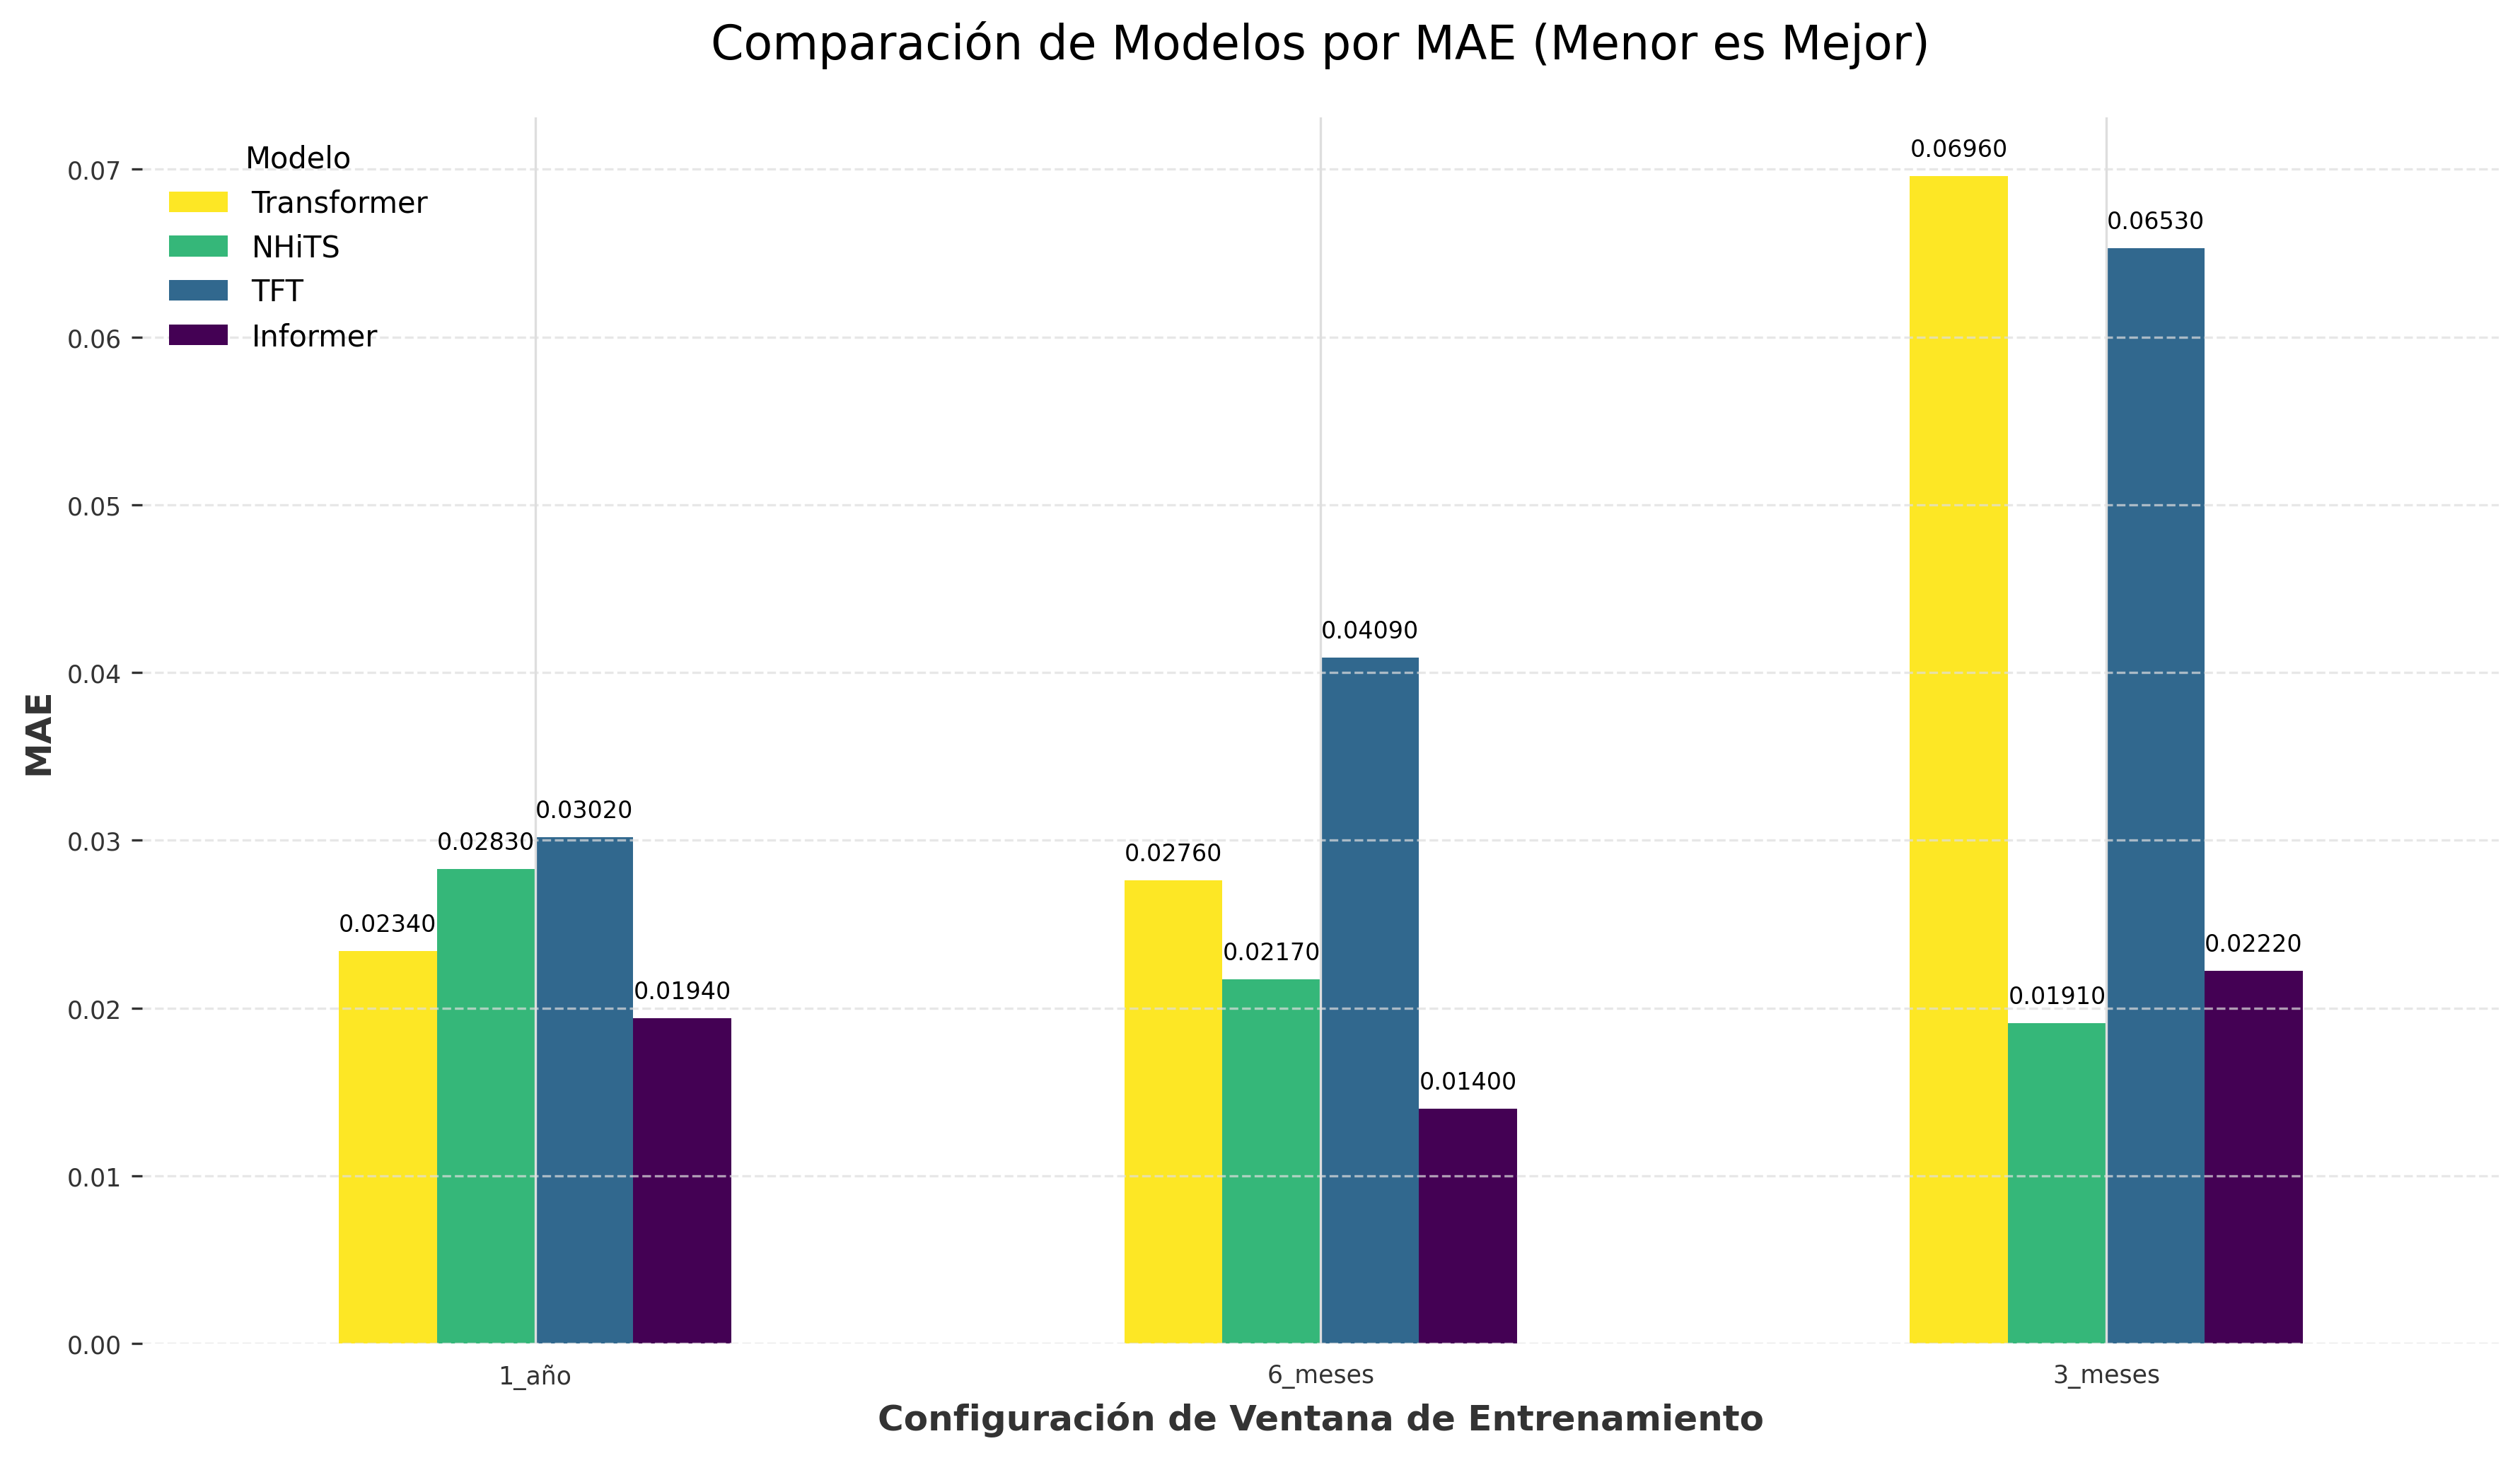
\includegraphics[width=0.85\textwidth]{./results/comparacion_modelos_por_MAE.png} 
\caption{Comparativa MAE vs ventana de entrenamiento.}
\label{mae}
\end{figure}

\begin{figure}[H] 
\centering
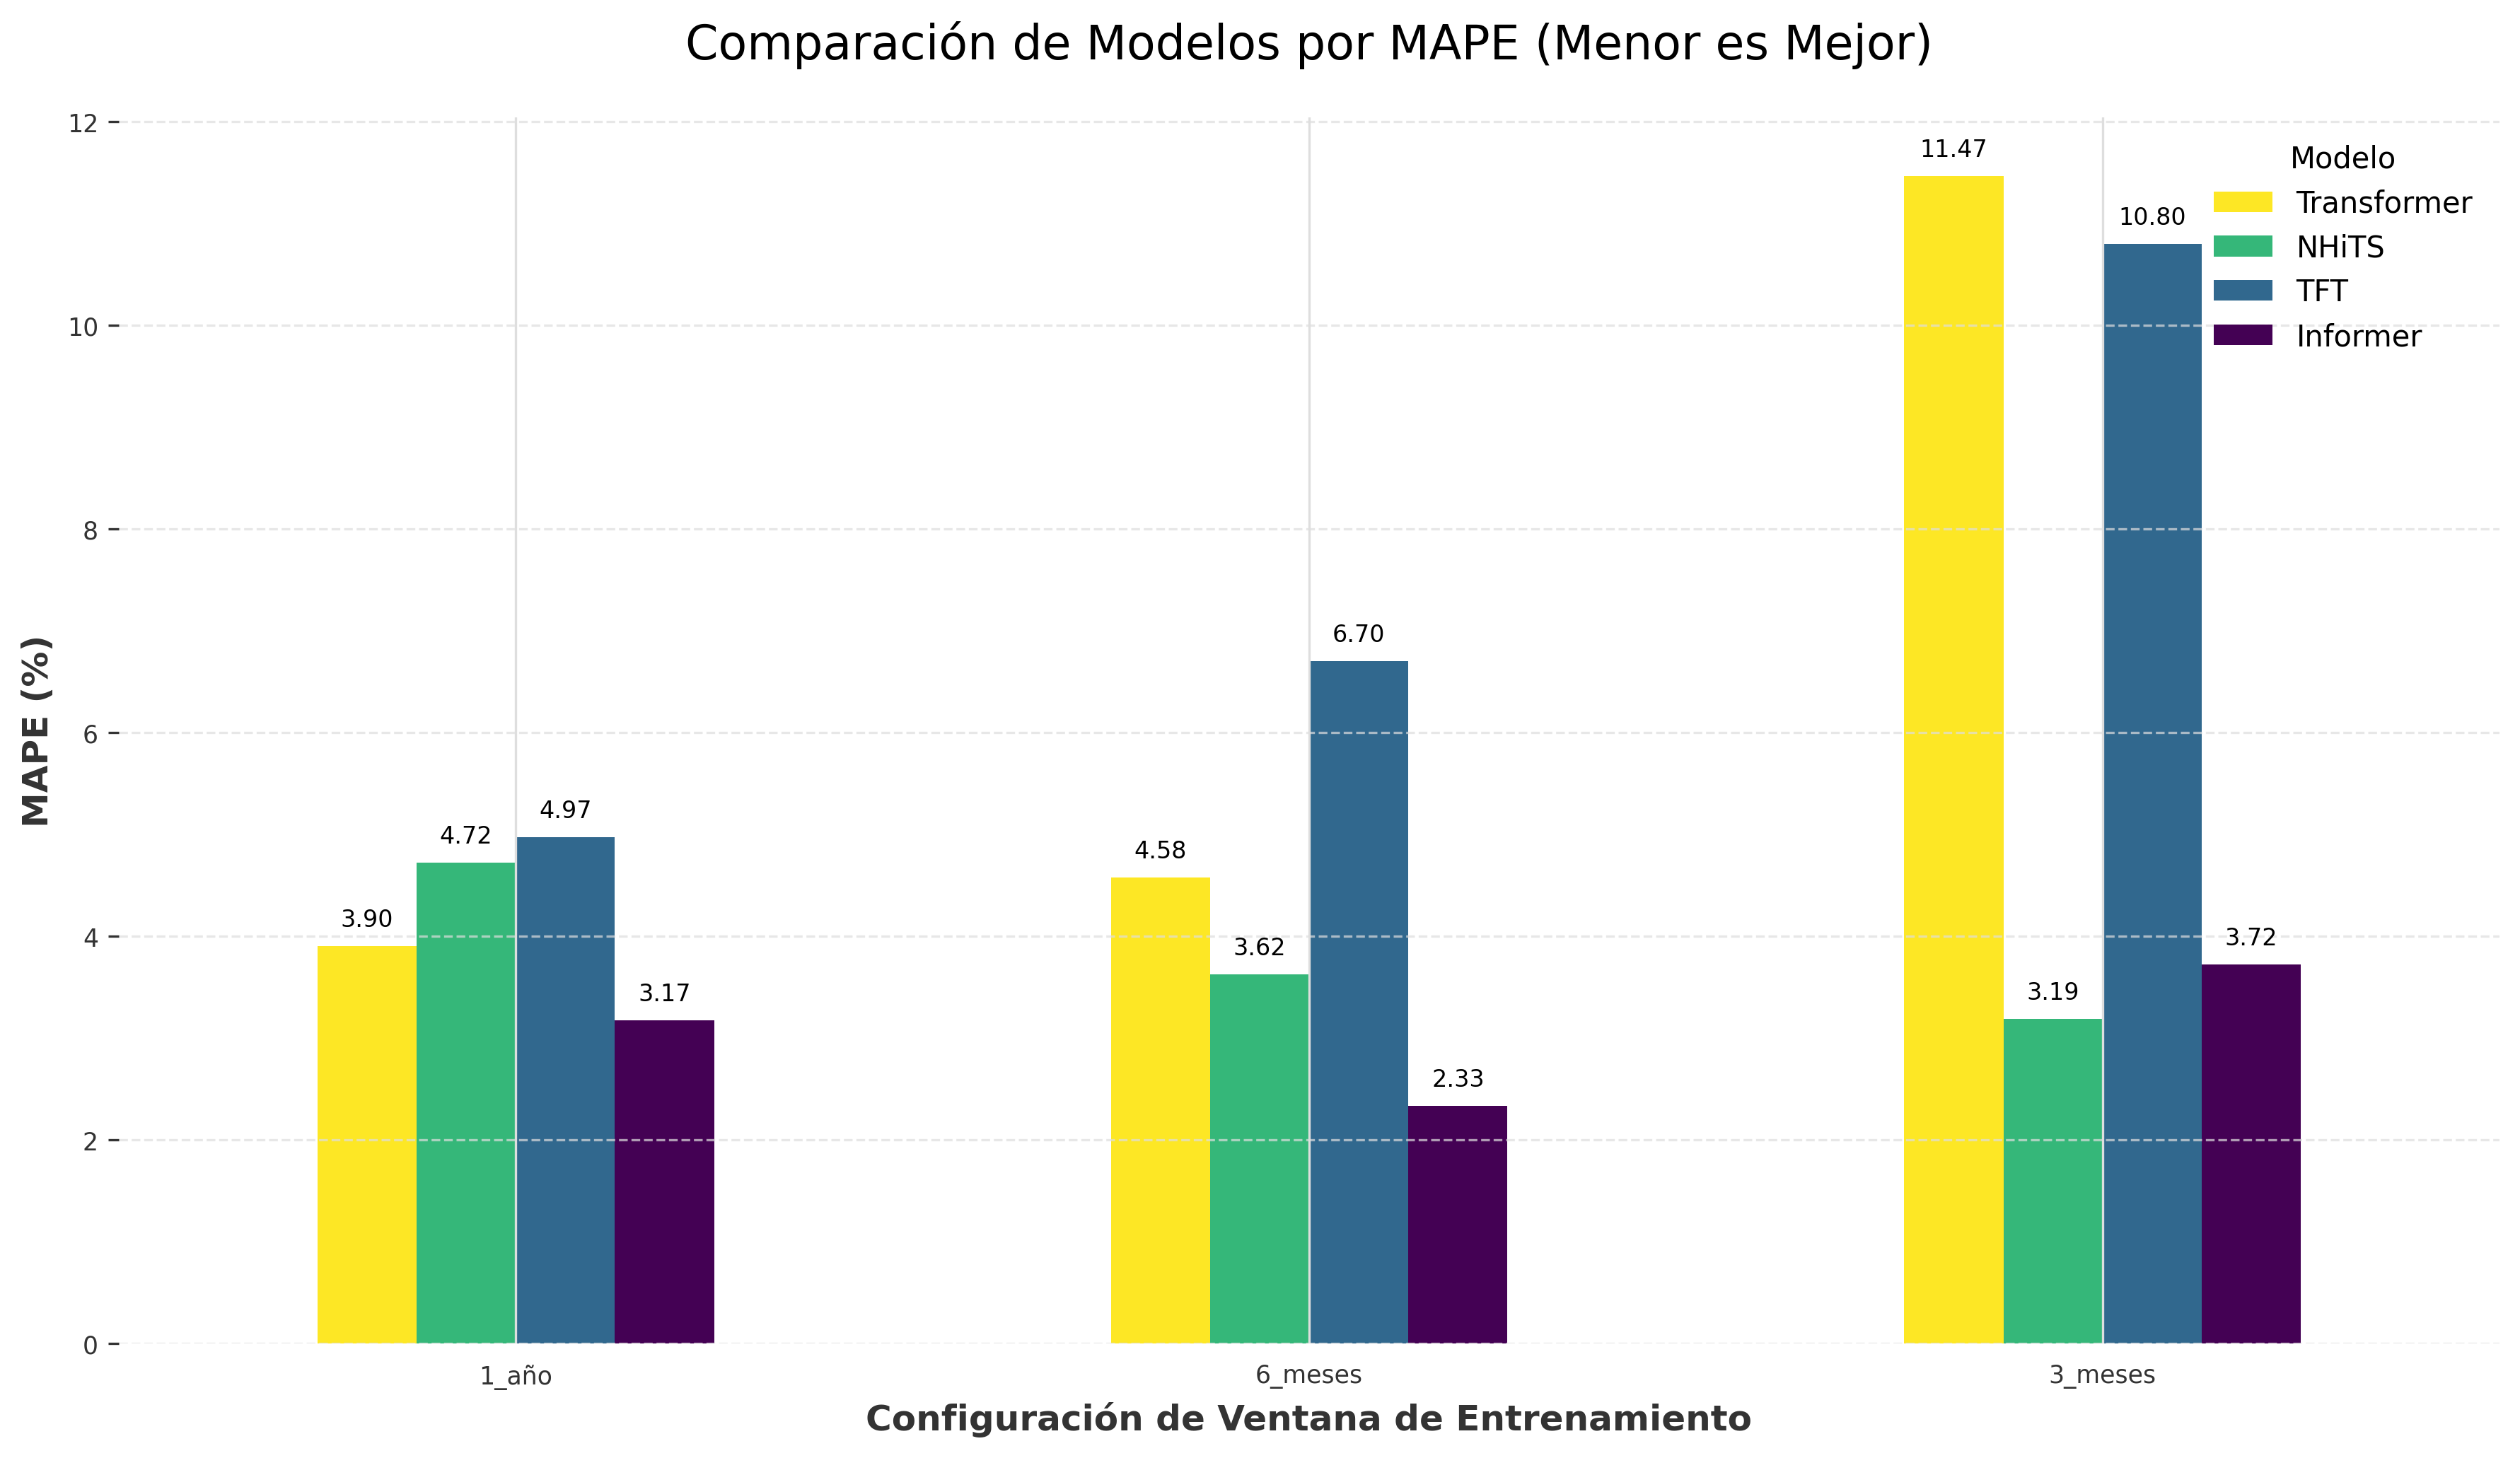
\includegraphics[width=0.85\textwidth]{./results/comparacion_modelos_por_MAPE.png} 
\caption{Comparativa MAPE vs ventana de entrenamiento.}
\label{mape}
\end{figure}

\begin{figure}[H] 
\centering
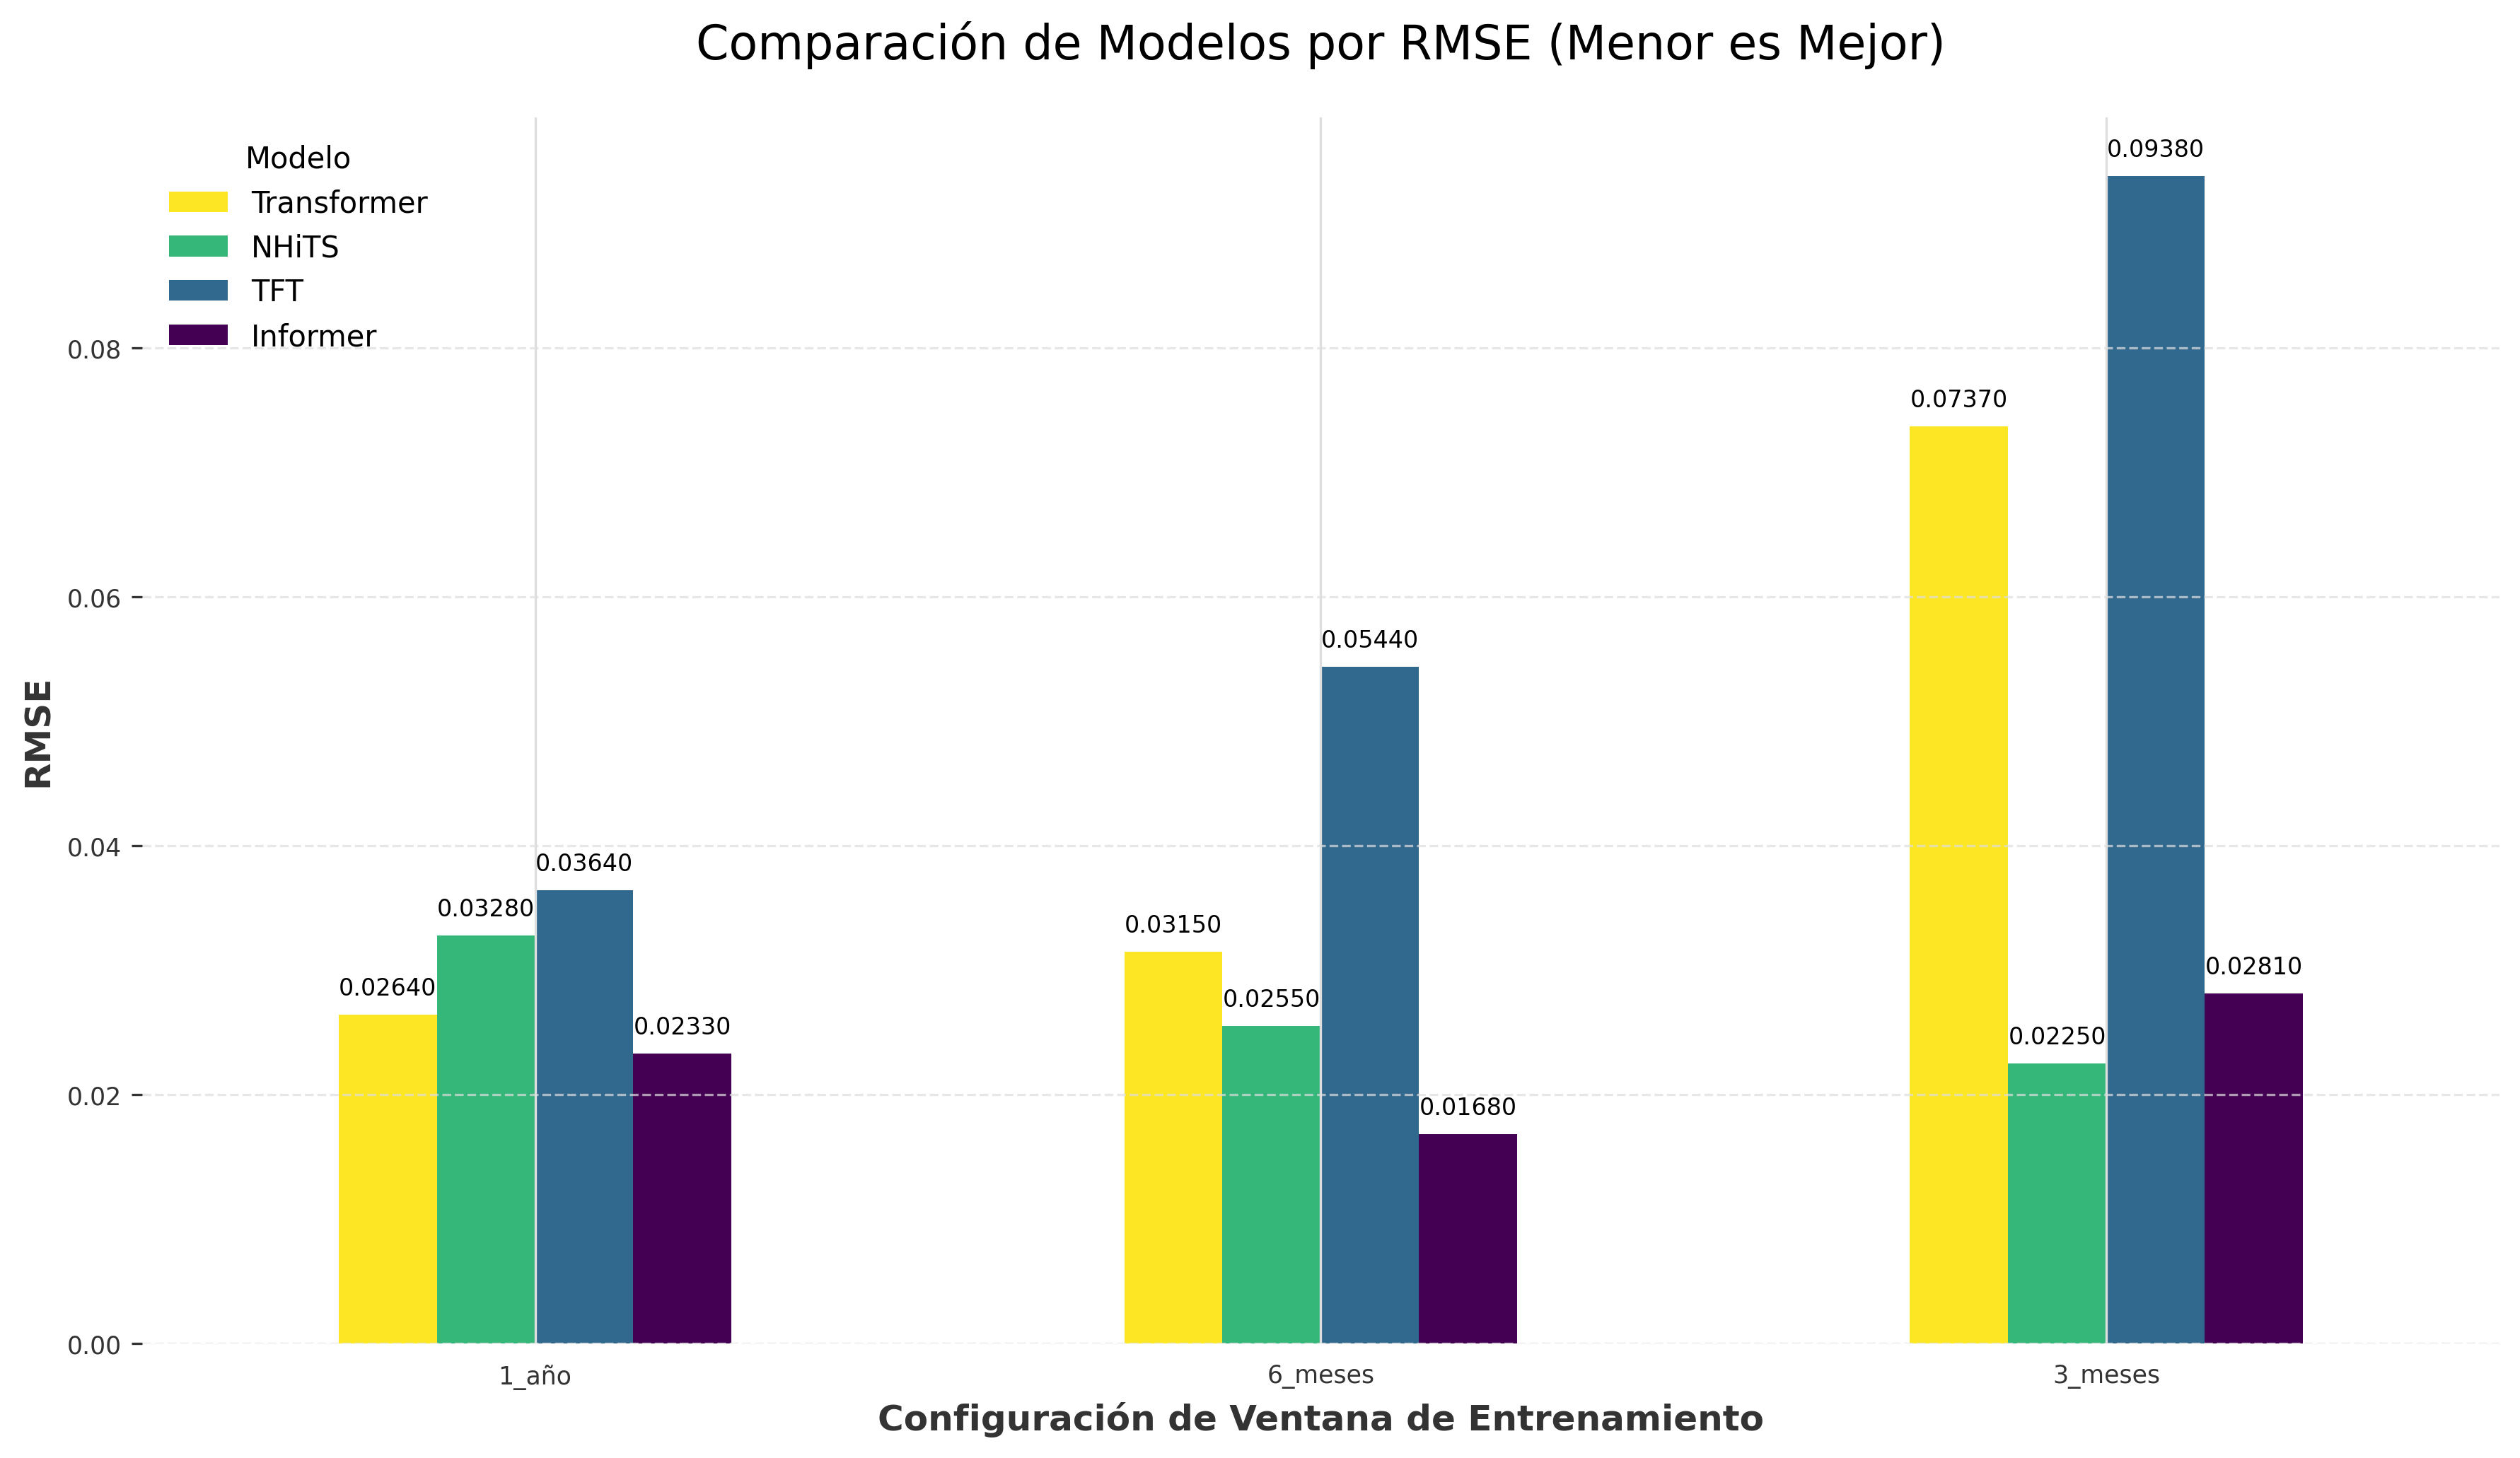
\includegraphics[width=0.85\textwidth]{./results/comparacion_modelos_por_RMSE.png} 
\caption{Comparativa RMSE vs ventana de entrenamiento.}
\label{rmse}
\end{figure}


\subsection{Predicciones de los diferentes modelos}

En las figuras \ref{prediccion_tres_meses} a \ref{prediccion_un_anio} se podrán observar las predicciones de los modelos evaluados en este trabajo.

\begin{figure}[H] 
\centering
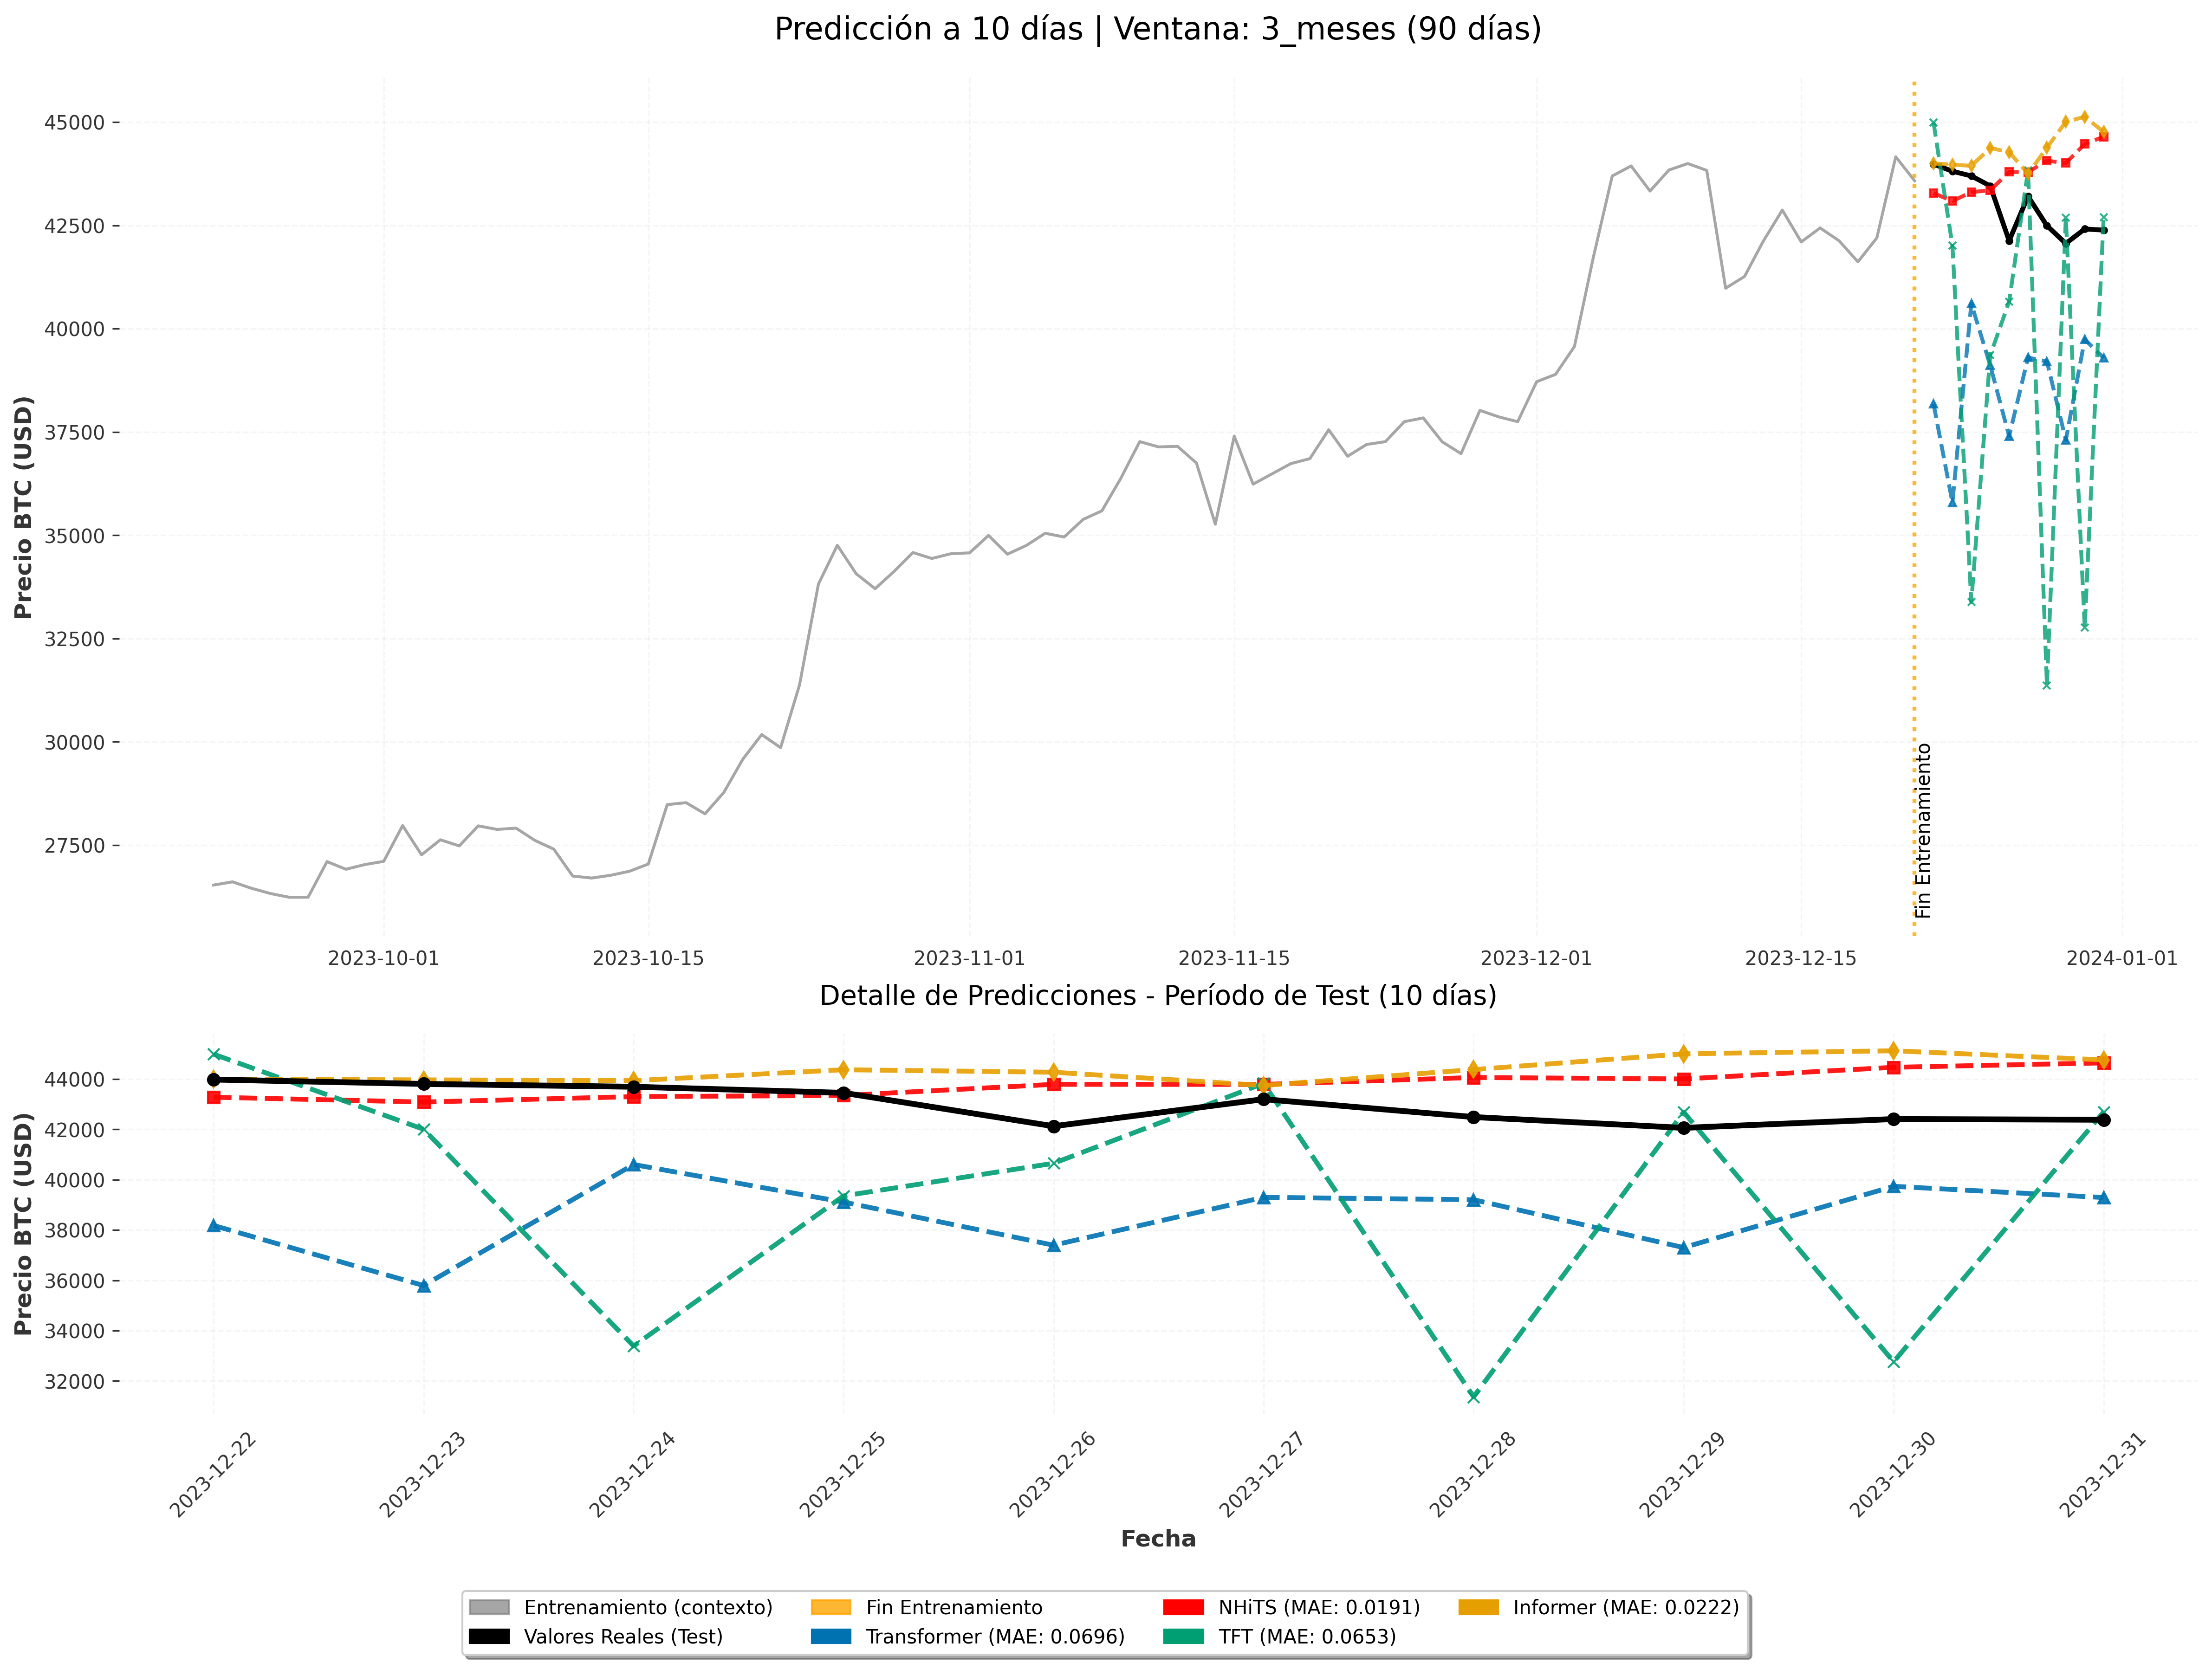
\includegraphics[width=0.85\textwidth]{./results/prediccion_bitcoin_3_meses_10dias.png} 
\caption{Predicciones vs Real a 10 días - ventana de entrenamiento 3 meses}
\label{prediccion_tres_meses}
\end{figure}

\begin{figure}[H]
\centering
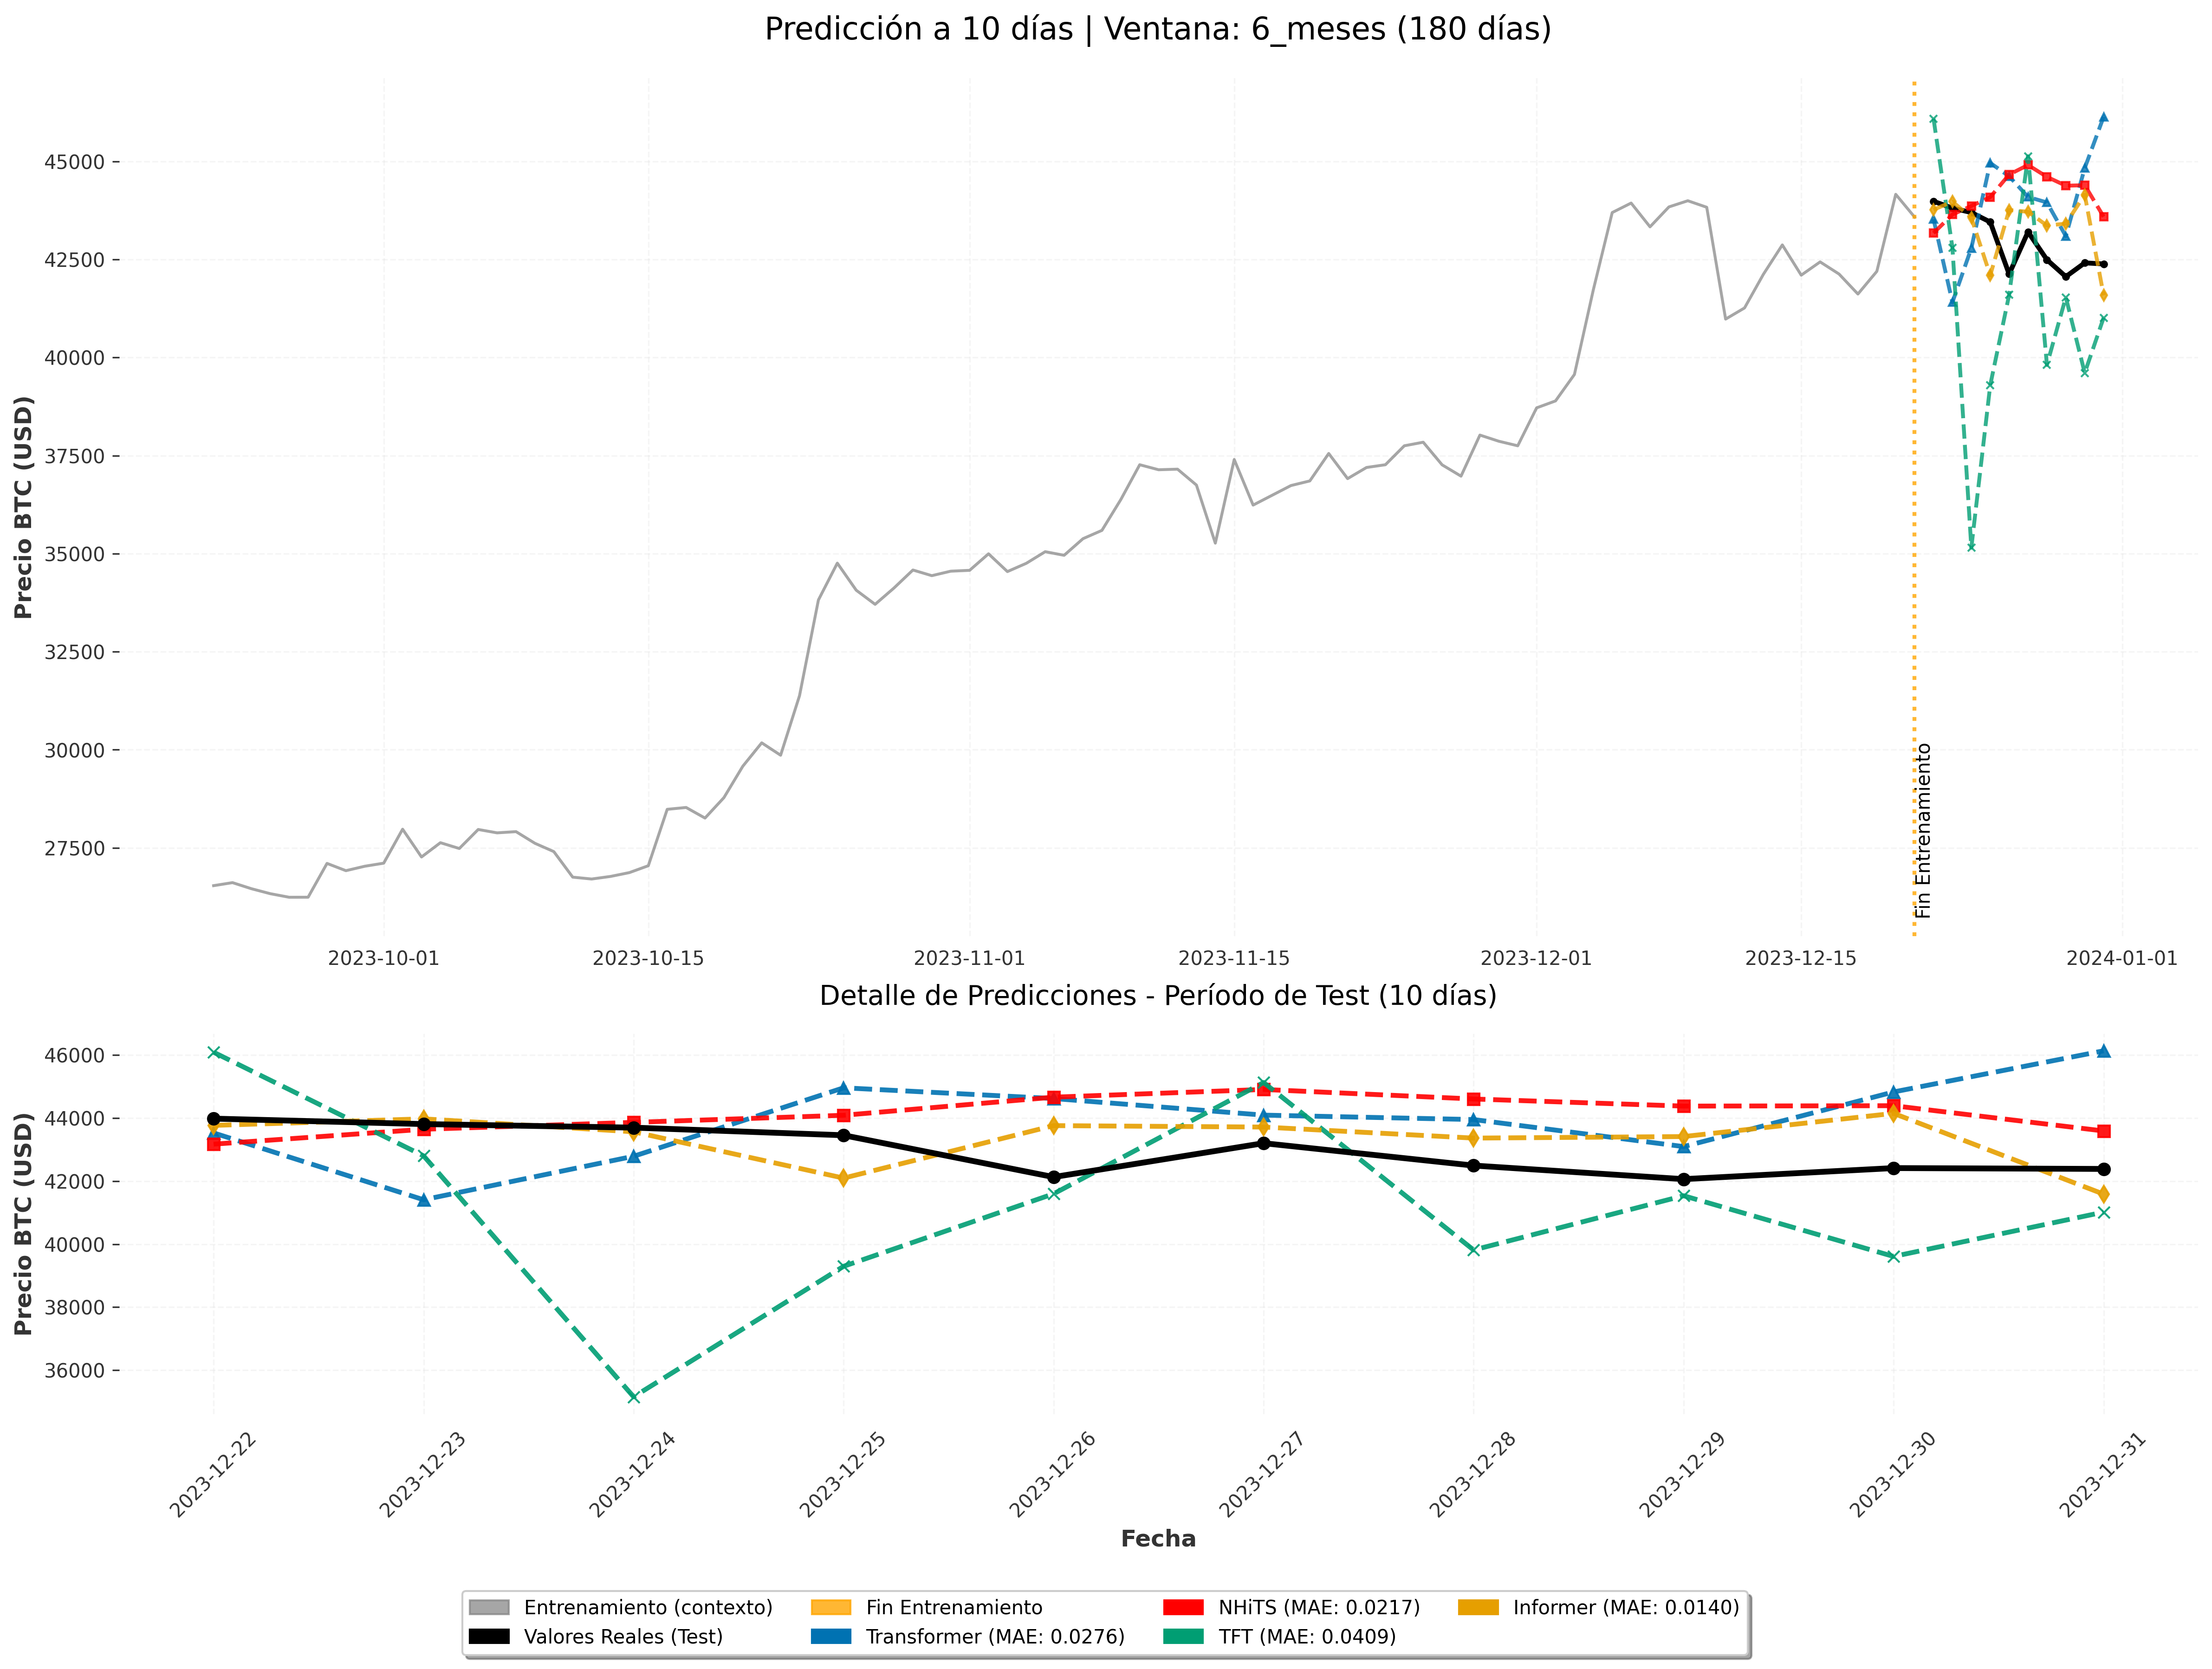
\includegraphics[width=0.85\textwidth]{./results/prediccion_bitcoin_6_meses_10dias.png} 
\caption{Predicciones vs Real a 10 días - ventana de entrenamiento 6 meses}
\label{prediccion_seis_meses}
\end{figure}

\begin{figure}[H]
\centering
\includegraphics[width=0.85\textwidth]{./results/prediccion_bitcoin_1_año_10dias.png}
\caption{Predicciones vs Real a 10 días - ventana de entrenamiento 1 año}
\label{prediccion_un_anio}
\end{figure}



%%%%%%%%%%%%%%%%%%%%%%%%%%%%%%%%%%%%%%%%%%%%%%%%%%%%%%%%%%%%%%%%%%%%%%%%

\newpage
\section{Conclusiones}
\label{sec:conclusiones}

\subsection{Hallazgos Clave}

\begin{itemize}
\item Los modelos Informer y NHiTs demostraron un rendimiento superior consistente en comparación con los demás modelos evaluados (TFT y Transformer), obteniendo los mejores resultados en todas las métricas de evaluación consideradas en este estudio: MAE, MAPE y RMSE.
Esta superioridad puede atribuirse a las innovaciones arquitectónicas específicas de cada modelo. El Informer destaca por su mecanismo ProbSparse self-attention que reduce significativamente la complejidad computacional mientras mantiene la capacidad de capturar dependencias de largo plazo en series temporales extensas. Por su parte, NHiTs aprovecha su arquitectura jerárquica de interpolación que permite una descomposición eficiente de las series temporales en múltiples escalas temporales, capturando tanto patrones locales como tendencias globales.
Los resultados sugieren que estas arquitecturas más recientes han logrado abordar efectivamente las limitaciones de los modelos Transformer tradicionales y TFT en el contexto específico del pronóstico de series temporales, ofreciendo no solo mayor precisión sino también mejor eficiencia computacional.
\item Los modelos evaluados presentaron limitaciones significativas durante eventos de alta volatilidad, evidenciando una disminución notable en la precisión de las predicciones cuando las series temporales experimentaron cambios abruptos o patrones irregulares.
\item La arquitectura de atención demostró ser particularmente efectiva para capturar dependencias a largo plazo
\end{itemize}

\subsection{Limitaciones y Trabajo Futuro}

\begin{itemize}
\item \textbf{Limitaciones}:
\begin{itemize}
\item Sensibilidad a cambios bruscos de tendencia
\item Dependencia de hiperparámetros
\end{itemize}

\item \textbf{Mejoras propuestas}:
\begin{itemize}
\item Incorporar datos de redes sociales (sentiment analysis)
\item Ensamblar múltiples modelos
\item Incluir datos de inflación, políticas monetarias, y correlaciones con mercados tradicionales
\end{itemize}
\end{itemize}

%%%%%%%%%%%%%%%%%%%%%%%%%%%%%%%%%%%%%%%%%%%%%%%%%%%%%%%%%%%%%%%%%%%%%%%%

\newpage
\section*{Anexo}
El código completo se encuentra disponible en: \\
\url{https://github.com/BenjaSar/AdST2}

\end{document}